\section{فعال نمودن قابلیت ها}
در حال حاضر قابلیت های مختلف را میتوانید چند بار تست کنید. نرم افزار بعد از هر بار استفاده تعداد مجاز باقیمانده را به شما یادآوری میکند. بعد از اینکه این سقف تمام شد،
در صورت تمایل به استفاده، میتوانید مطابق پنچره راهنما (مطابق شکل 
\ref{pic:register}
) کدی که نرم افزار به شما میدهد را به همراه فیش واریزی، برای من ارسال کنید. من در اسرع وقت  قابلیت مورد نظر شما را فعال میکنم و به شما اطلاع میدهم. بعد از آن کافیست یکبار در حالی که به اینترنت متصل هستید قابلیت مورد نظرتان را اجرا کنید تا این قابلیت برای شما فعال شود.

 
 \begin{figure}
     \centering
     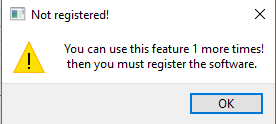
\includegraphics[scale=0.7]{figures/no_of_using}
     
\includegraphics[scale=0.8]{figures/register}
     \caption{توضیح چگونگی فعال کردن قابلیت مورد نظر در نرم افزار}
     \label{pic:register}
 \end{figure}
 
